\chapter{绪论}
\section{研究背景与意义}
在自然界,外骨骼是一种能为生物内部组织和器官提供保护的外部结构,如虾、蟹、昆虫等节肢动物体表坚韧的几丁质的骨骼。近些年的科幻电影中,频繁出现一些能够提高人体机能的可穿戴外骨骼,如《钢铁侠》中的Mark战甲、《流浪地球》中救援队的作战装甲等。

实际上,外骨骼机器人并非仅存于幻想,其在人体运动机能提升\cite{p1}和医疗康复\cite{p2}领域的研究已存在超过半个世纪。外骨骼机器人是一种综合传感技术、信号处理、智能控制、人机交互的一体化可穿戴机械装置。随着机器人技术的发展,传统的独立作业机器人,如工业机器人、无人机等,已相对成熟,而具有人机协同功能的机器人成为研究热点。外骨骼机器人作为其典型的应用,正逐渐受到研究人员的重视。近些年随着检测技术、控制理论、人工智能等相关领域的发展,可穿戴设备的研究取得了巨大的进步。

在现代战争士兵需要背负越来越多的武器和设备,进行远距离机动和长时间作战,其体力和耐力受到严重考验。使用助力外骨骼可以有效减轻士兵负担,从而提高单兵作战能力和战场生存能力。另一方面,随着人口老龄化趋势的增加和人们健康意识的提高,医疗康复设备的需求量日益增长。下肢外骨骼机器人能够使残疾人和老年人重新获得行走与生活自理能力,从而减轻对家庭和社会的负担。

下肢外骨骼的研究主要聚焦于三个方向:一是为正常人设计、旨在提高人体运动机能的助力设备,其主要应用于军事作战、抢险救灾和工业负重;二是为运动障碍者设计的助力设备,穿戴者可以在外骨骼的辅助下重新获得行走能力;三是可穿戴式康复医疗设备,旨在通过预先设定的重复性动作帮助患者恢复身体机能。本项目研究脚踝式助力外骨骼,通过在运动过程中为穿戴者提供关节力矩辅助,从而减轻穿戴者的运动负担,提高穿戴者的运动机能。

\section{外骨骼机器人的研究现状}

\subsection{国外研究现状}
\begin{figure}[!h]
    \label{fig:sub1}{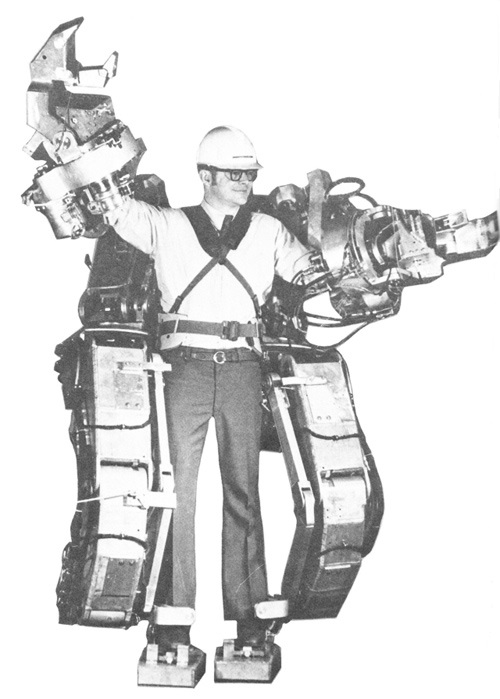
\includegraphics[width=4.2cm]{fig/f3_Hardiman.jpg}}\quad
    \label{fig:sub2}{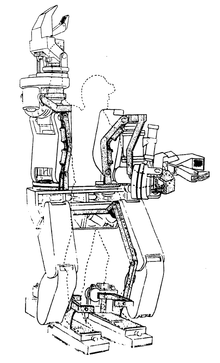
\includegraphics[width=3.8cm]{fig/f4_Hardiman.jpg}}
    \caption{通用公司研制的全身型外骨骼机器人Hardiman\cite{p6}}
    \label{fig:subfigs}
\end{figure}

上世纪60年代晚期,美国通用公司与康奈尔大学的研究人员联合研制了一种全身驱动的外骨骼机器人Hardiman\cite{p6}。其拥有30个自由度,整机重量650Kg,关节由液压驱动,可以放大穿戴者25倍的重量。这项工作最先尝试了外骨骼设计的驱动选型与人机交互等问题,并由此开创了外骨骼机器人的研究。
\begin{figure}[htb]
    \subfloat[下肢助力外骨骼BLEEX\cite{p5,p7}]{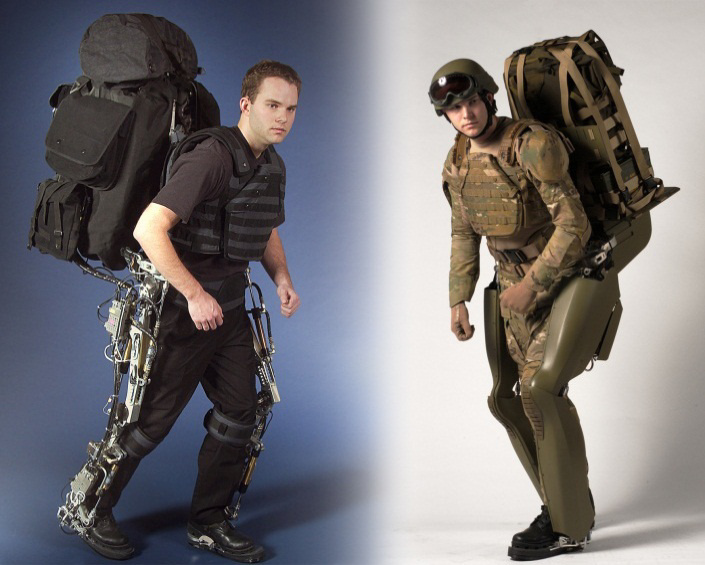
\includegraphics[width=7.9cm]{fig/f5_BLEEX.jpg}}\quad
    \subfloat[下肢康复外骨骼Ekso\cite{p9}]{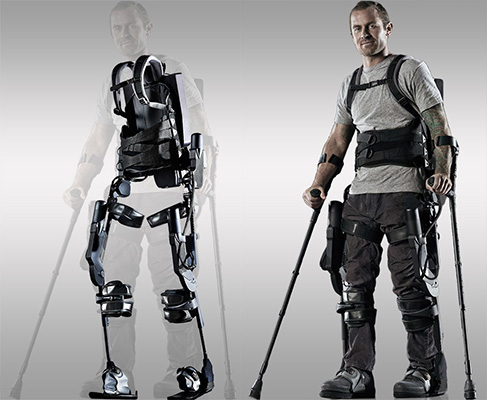
\includegraphics[width=7.7cm]{fig/f9_ekso.jpg}}
    \caption{伯克利大学研发的外骨骼机器人}
    \label{fig:subfigss}
\end{figure}

从2000年开始,美国先进国防项目研究署(DARPA)开始了“增强人体机能的外骨骼项目”(EHPA),计划研制一种外骨骼,用以提高士兵的军事作战能力。其中最为知名是美国加州伯克利大学分校的研究人员研制的BLEEX\cite{p5,p7}(Berkeley Lower Extremity Exoskeleton)。BLEEX下肢外骨骼机器人自重50Kg,驱动采取液压驱动,结构上采用拟人的设计方式,每条腿共有7个自由度:髋关节3自由度,膝关节1自由度,踝关节3自由度。穿戴时负载能够通过外BLEEX骨骼传递到地面从而减轻穿戴者的负重感,在负重34Kg时穿戴者的感受仅为2Kg。

在BLEEX项目进行的同时,项目团队也对医用下肢外骨骼进行了研究,并于2010年推出了eLEGS\cite{p9},后改名为Ekso。Ekso下肢外骨骼系统能够帮助下肢截瘫患者重新获得行走能力,并在长期训练后可以恢复患者的运动。目前Ekso已经获得美国食品和药物管理局的认证,在美国多个医院和医疗机构中用于截瘫患者的康复治疗。
\begin{figure}[htb]
    \label{fig:sub1}{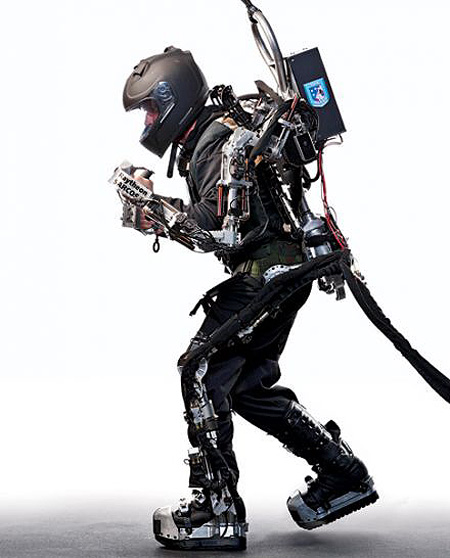
\includegraphics[width=6.5cm]{fig/f6_XOS.jpg}}\quad
    \label{fig:sub2}{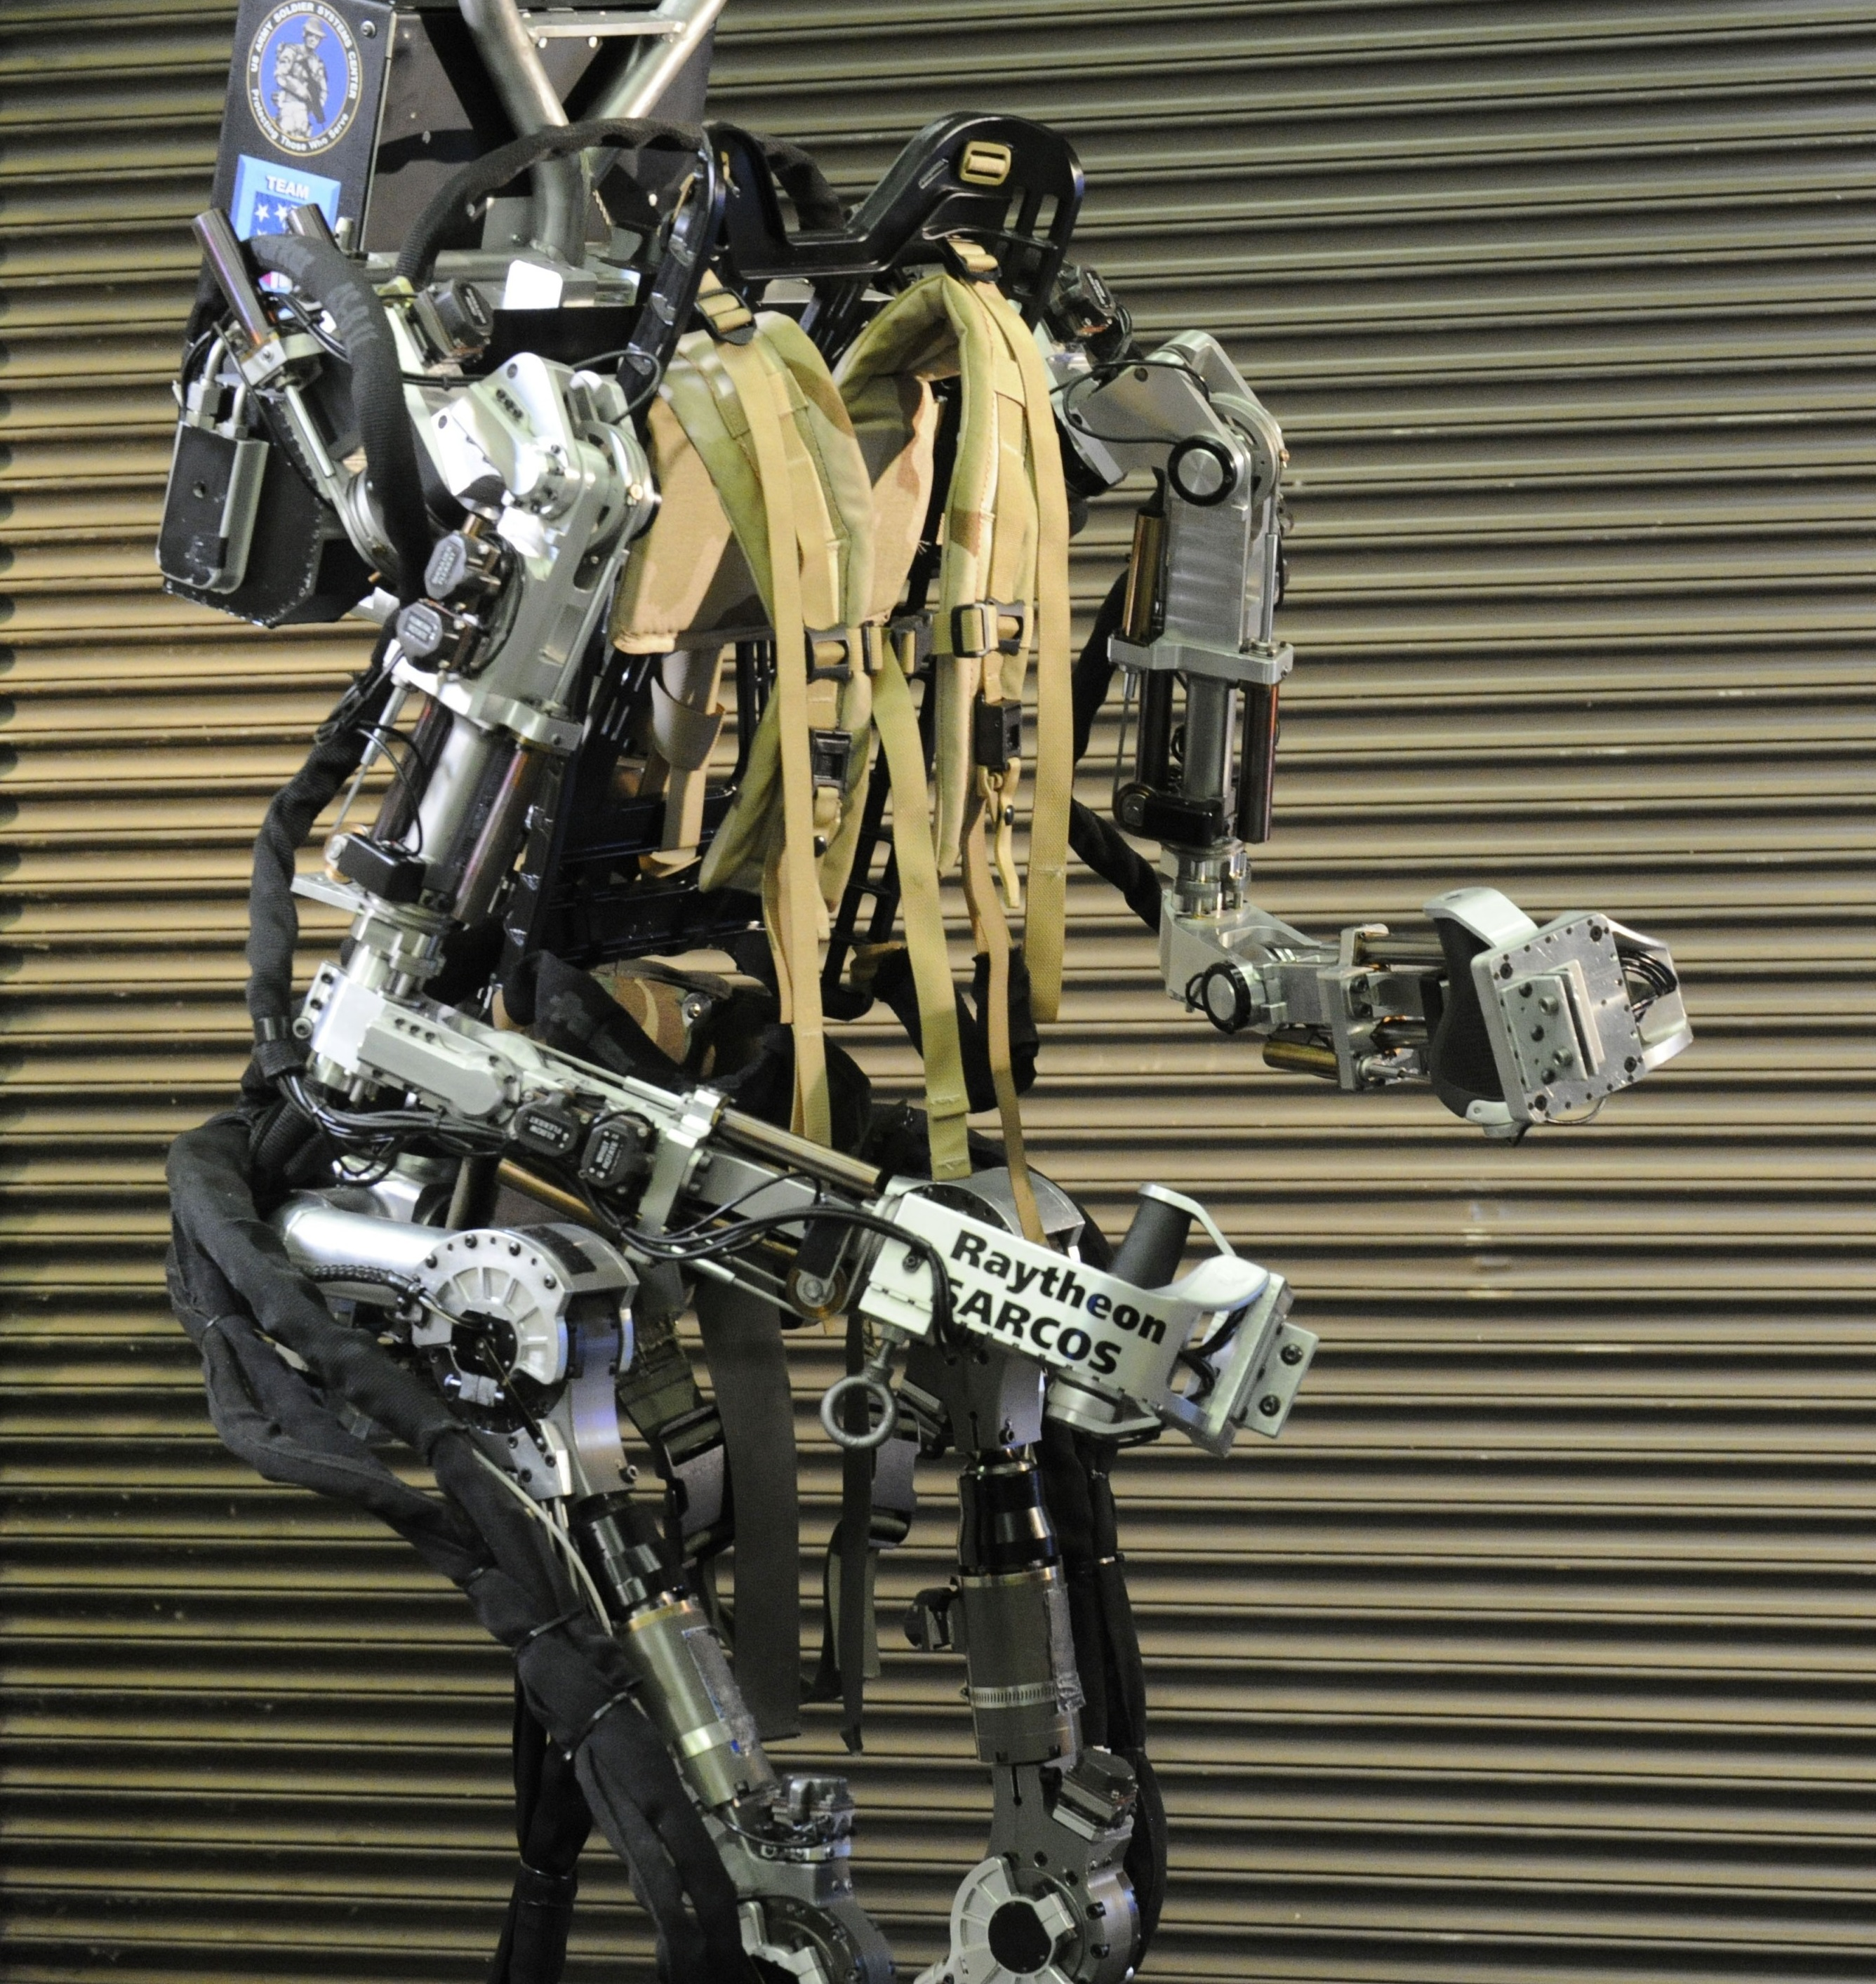
\includegraphics[width=7.5cm]{fig/f7_XOS.jpg}}
    \caption{XOS2全身型军用外骨骼\cite{p8}}
    \label{fig:subfigs}
\end{figure}

另一个受到DARPA EHPA支持的项目为美国雷神公司的XOS\cite{p8}。XOS为全身型的助力外骨骼,关节采用液压驱动,能够帮助穿戴者在负重90Kg的情况下进行长时间的运动。XOS外骨骼的自由度非常多,可以灵活的完成跑、跳,甚至是俯卧撑、拳击、踢足球等运动。但XOS对供电的需求非常大,自身携带的电池仅能运转40分钟,测试时必须拖着一条电缆进行供电,因此并不是完全的可穿戴设备。

除了伯克利系列的下肢外骨骼外,其他科研机构也研究出各具特色的外骨骼。麻省理工学院研究了一种下肢负重外骨骼MIT Exoskeleton\cite{p11},驱动上采用了串联弹性驱动SEA(Series Elastic Actuator),能够使穿戴者在负重36kg的情况下依然可以顺畅运动。哈佛大学的研究人员针对刚性的外骨骼系统质量大、穿戴不舒适等问题,研制出一种柔性外骨骼\cite{p12},采用鲍登线与身体各部分的锚点相连,电机转动时拉动锚点,从而带动肢体运动。日本筑波大学研发了混合助力机器人HAL\cite{p13}(Hybrid Assistive Limb),用于帮助脊柱损伤患者和中风病人。其采用基于肌电信号的控制方法,可以有效降低肌肉的使用率。
\begin{figure}[htb]
    \subfloat[哈佛大学的柔性外骨骼Soft-Exosuit\cite{p12}]{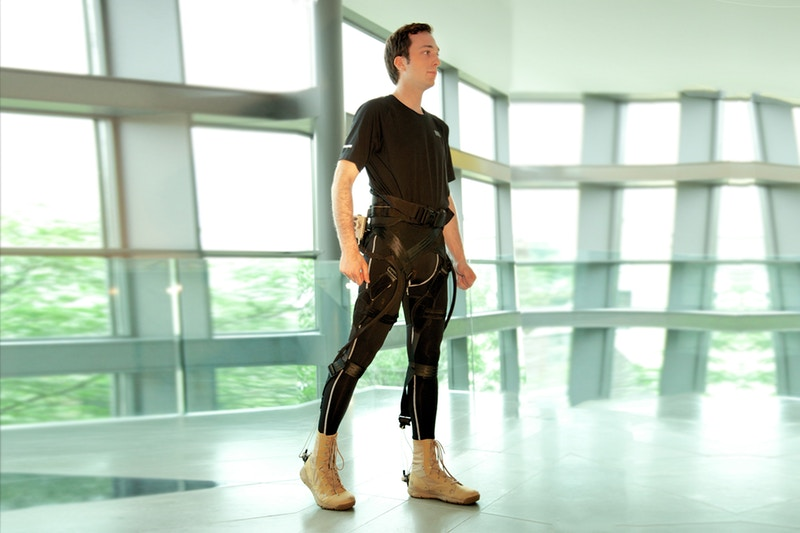
\includegraphics[width=7.8cm]{fig/f10_soft.jpg}}\quad
    \subfloat[康复型外骨骼HAL\cite{p13}]{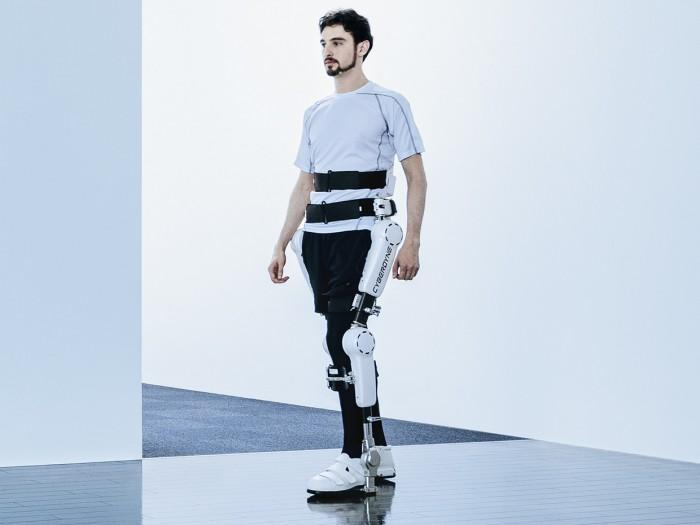
\includegraphics[width=7cm]{fig/f12_hal.jpg}}
    \caption{其他研究机构研发的助力外骨骼}
    \label{fig:subfigss}
\end{figure}

\subsection{国内研究现状}

国内助力外骨骼的研究起步相对较晚,但经过十几年的发展,相关技术已经逐步接近国际水平。
\begin{figure}[!htb]
    \subfloat[中科院智能所研制的WPAL\cite{p16}]{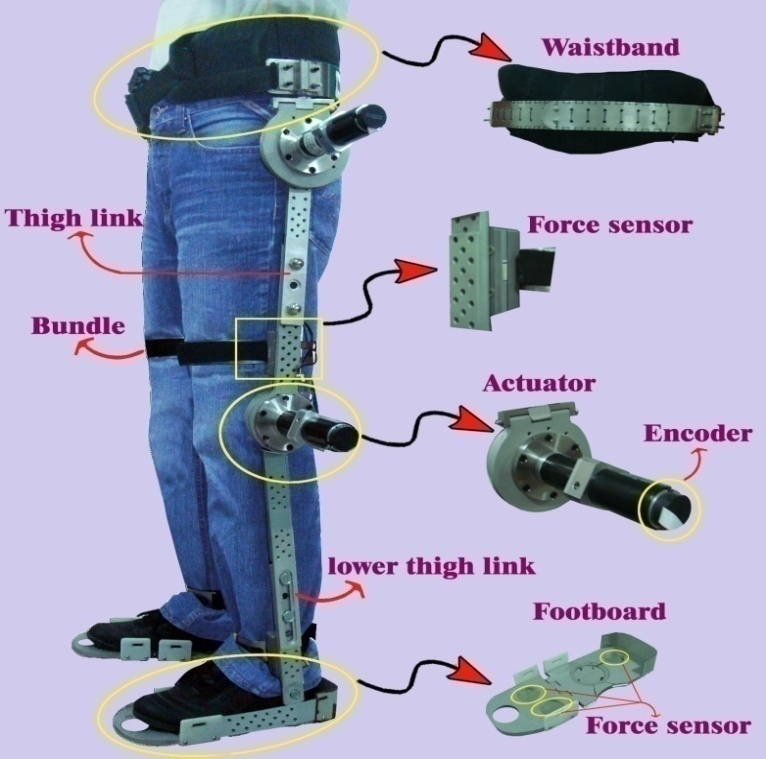
\includegraphics[width=6.5cm]{fig/f13.jpg}}\quad
    \subfloat[哈工大研制的HIT-LEX\cite{p18}]{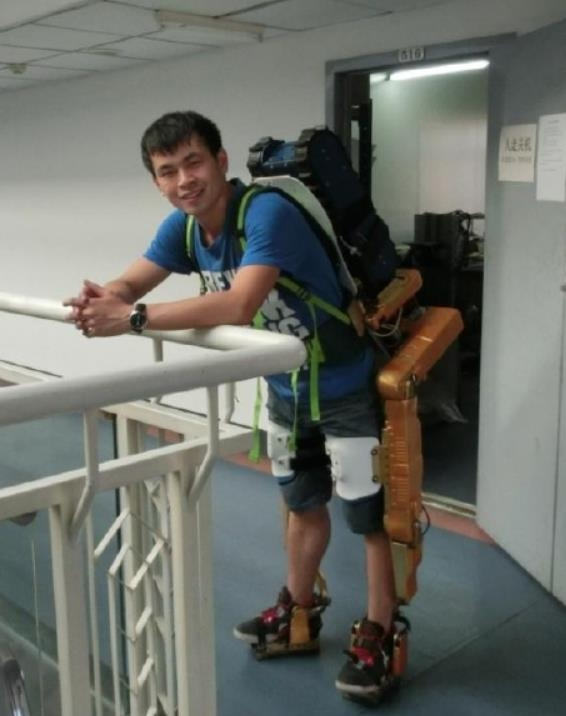
\includegraphics[width=5cm]{fig/f15.jpg}}\\
    \subfloat[浙大研制的气动外骨骼\cite{p17}]{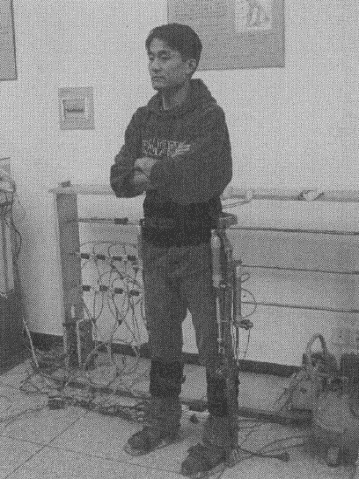
\includegraphics[width=5cm]{fig/f16.jpg}}\quad
    \subfloat[202所研制的助力外骨骼]{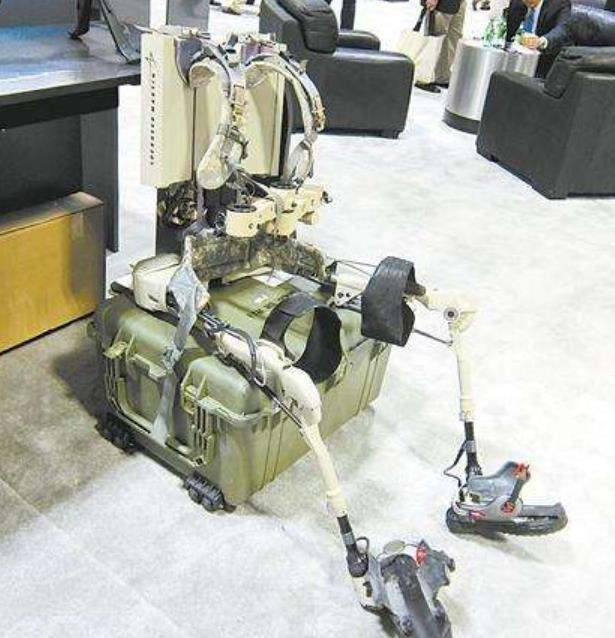
\includegraphics[width=6.5cm]{fig/f17.jpg}}
    \caption{国内高校和机构研发的外骨骼机器人}
    \label{fig:subfigss}
\end{figure}

中科院合肥智能所的余勇研究员和葛运建研究员早在2004年就带领团队研究出了下肢助行外骨骼WPAL\cite{p14}( Walking Power Assist Leg)。WPAL能够通过足底压力传感器获取穿戴者的运动负重,并调整其模型和控制器中的参数,从而提高外骨骼的负重效率\cite{p15}。

哈尔滨工业大学的朱延河教授于2013年带领团队研制了一款下肢助力外骨骼HIT-LEX\cite{p18}。该外骨骼主要为抢险救灾的救援人员所设计,在机械结构上和BLEEX一样采用拟人化设计,在后背与足底均装有压力传感器用来检测穿戴者的运动意图。经测试,该外骨骼最大负重50kg,续航距离5km,续航时间2h。

成都电子科技大学研发了一种电机驱动的下肢外骨骼机器人,并且设计了分布式的控制系统,由低层感知与上层控制器相结合,使用灵敏度放大的控制方法对系统进行整体控制\cite{p19}。

浙江大学采用气动系统设计了一种新型的下肢助力外骨骼,并基于自适应模糊神经网络进行控制,对人机耦合控制策略进行了研究\cite{p17};上海交通大学研究了一款基于混联结构的下肢外骨骼机器人,该机器无膝关节,通过储能式弹簧降低关节利用\cite{p20};此外,中国兵器工业集团202所、航天科工二院206所、中国兵器工业集团208所等,都对助力外骨骼进行了研究。

\section{外骨骼控制方法的研究现状}

早期的外骨骼系统大多使用位置轨迹追踪的控制方法\cite{p21,p22},但位移控制在人机动作不一致时会产生大的作用力,从而产生人机交互的安全风险。因此外骨骼控制正越来越多的从单纯的轨迹控制,转向对穿戴者动作反应更加柔和的力矩控制。这不仅出于安全性与舒适型的考量,也包含了对人体动力学更深刻的理解\cite{p23,p24}。

经典的PID反馈控制方法和其变化形式,由于简单、实用的特点,被广泛的应用到外骨骼系统的控制中。积分控制模块用于减小稳态误差,在低阻抗的外骨骼中有较好效果\cite{p25}。在系统阻抗较高且模型不确定的情况下,PD控制更为合适\cite{p27,p28}。基于模型的控制方法经常用来提高力矩追踪的性能,典型的有使用逆动力学模型的前馈力矩补偿\cite{p29},但这种方法只有在模型准确的时候才有较好的效果。自适应控制也被用到外骨骼系统中,例如基于SEA的被动控制方法\cite{p30}。迭代学习方法也被应用到腿式机器人的运动控制中\cite{p31},这种方法通过一步一步的迭代来学习并消除误差,对于周期性轨迹的跟踪比积分控制有更好的效果。

在实际的应用中,力矩控制一般由底层控制器和上层控制器组成。底层控制器(如PID控制器)用来控制驱动器对期望关节力矩进行追踪,而顶层控制器用来产生期望的关节力矩。在这种控制策略中,期望力矩并不是事先选定好的控制目标,而是由人机交互过程中产生的动态信号。典型的上层控制器有直接力矩控制、阻抗控制、灵敏度放大控制和EMG信号控制方法。

直接力矩控制是最为简单的上层控制器形式,通过一个关于时间的函数来生成期望力矩曲线\cite{p32,p33},这里时间一般为步态周期百分比而非绝对时间。直接力矩控制只在稳定运动下才能产生有效的助力效果,并且其曲线参数对个体、环境的变化较为敏感,需要针对不同实验条件进行精心调整。阻抗控制模仿了正常人类行走时关节角度与关节力矩的关系,根据关节角度来生成期望力矩\cite{p34}。它是典型的柔顺顺控制方法,具有较好的人机交互性,对扰动和不确定性有很好的鲁棒性。但是由于在控制过程中很难得到精确的位置轨迹,所以使得其控制精度有所欠缺。灵敏度放大控制是加州伯克利大学应用于BLEEX外骨骼的控制方法\cite{p35},它需要精确的动力学模型。当穿戴者施加较小力矩带动外骨骼运动时,系统感受到人体运动意图并通过外骨骼将此运动放大,使穿戴者感受到较小的运动阻力。但其依赖精确的模型,对不同个体的适应度较差。基于EMG信号的控制方法是通过测量穿戴者的EMG信号,使用前向动力学的方法估计出外骨骼所需要的施加的力矩,从而实现端到端的直接控制\cite{p36}。但这种方法对于环境和EMG信号测量的要求较高,且容易受穿戴者个体因素的影响。

这些上层的控制策略均在特定环境和条件下有较好的效果,但无论那种控制方法,均需要根据穿戴者的个体特性对控制参数进行调整,以达到最佳的助力效果。

\section{“人在环中”外骨骼优化方法的研究现状}

正如上节所述,由于人类个体之间生理学和神经学的差异,不同个体对同一个助力参数的反应大相径庭\cite{p37}。因此上层控制器的控制参数或助力模式需要根据个体差异进行调整。为了能够充分发挥外骨骼的潜力,控制器需要根据个体差异的不同,自动寻找其适合的助力模式,实时的调整控制策略使得穿戴者的身体机能达到最大值,这种方法被称为“人在环中”的优化方法\cite{p38}。
\begin{figure}[!htb]
    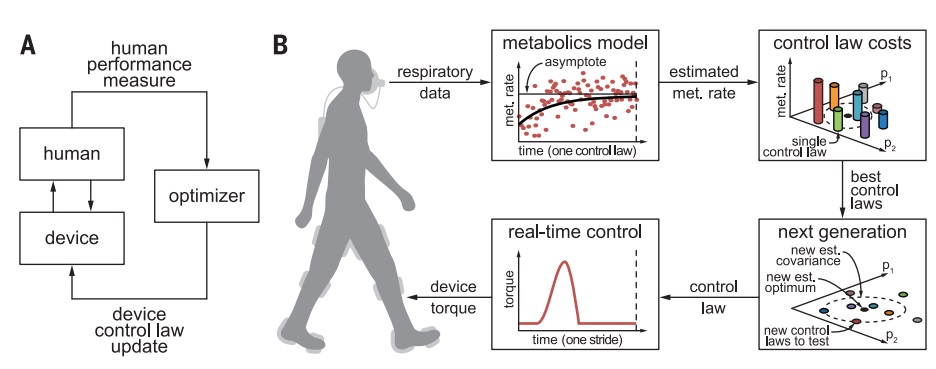
\includegraphics[width=15cm]{fig/f18.jpg}
    \caption{人在环中的参数优化方法\cite{p40}}
    \label{fig:mark}
\end{figure}

具体来说,人在环中优化以人体机能为反馈,以每个控制模式的控制器参数为优化对象,通过测量每组参数的生理反馈值,采用一定的优化算法找到适合个体的最佳参数,从而达到提高人体机能的目的。

“人在环中”的优化方法刚刚兴起,相关研究较少。最初的研究使用线性搜索\cite{p38}或梯度下降\cite{p39}的方法优化单个控制器参数,前者对于高维参数优化效率较低,而后者对噪声非常敏感。Zhang等人\cite{p40}使用自适应协方差进化算法优化踝关节外骨骼的四个控制参数,优化后穿戴者在常速行走状态下的代谢耗能下降了24\%。Ding等人\cite{p41}使用Bayesian优化算法对柔性髋关节外骨骼的两个控制参数进行优化。

人在环中的方法将穿戴者视为外骨骼系统的一部分。但目前以人体机能为反馈的人在环中优化还存在很多问题。基于人体代谢耗能的反馈虽然较为稳定,但测量时间较长,优化效率很低,优化过程容易导致人体疲劳。另外适用于人在环中优化的算法目前尚无定论。稳定且灵敏的人体反馈数据,快速而高效的优化算法,仍有待进一步研究。

\section{本文主要研究内容}

本文主要研究内容包括以下三个部分:

(1)搭建外骨骼的数据采集与处理系统。
针对所研究的踝关节式外骨骼,搭建了基于应变片的外骨骼力矩测量模块、基于足底开关的步态周期检测模块、基于EMG信号和肌肉激活度检测模块和基于IMU的人体姿态数据采集系统。

(2)设计外骨骼的力矩控制系统。
力矩控制由上层控制器与底层控制器组成,上层控制器用来产生期望力矩曲线,底层控制器实现对期望力矩曲线的跟踪。针对上层控制器,本文采用基于时间的直接力矩控制器,通过三次函数插值得到期望力矩曲线。针对底层控制器,本文提出了三种控制算法,设计了四种不同组合形式的控制器,并对其进行了验证与对比。

(3)研究“人在环中”的外骨骼优化方法。
由于个体差异性,最佳助力模式因人而异。为了充分发挥外骨骼的潜能,本文以穿戴者的肌肉激活水平为目标函数,使用贝叶斯优化外搜寻最佳助力参数。实验表明,外骨骼系统能够在五分钟内寻找到受试者的最佳助力参数。在优化后的助力参数下,受试者肌肉激活度平均下降12.2\%。